%%%%%%%%%%%%%%%%%%%%%%%%%%%%%%%%%%%%%%%%%%%%%%%%%%%%%%%%%%%%%%%%%%%%%%%%%%%%%%%
% Chapter 3: Procedimiento experimental 
%%%%%%%%%%%%%%%%%%%%%%%%%%%%%%%%%%%%%%%%%%%%%%%%%%%%%%%%%%%%%%%%%%%%%%%%%%%%%%%

%++++++++++++++++++++++++++++++++++++++++++++++++++++++++++++++++++++++++++++++
\section{Descripci�n de los experimentos}
\label{3:sec:1}

  El experimento llevado a cabo en esta memoria ha consistido en la realizaci�n de varios c�digos en lenguaje $Python$. Los algoritmos implementados que solucionan dichos c�digos 
estiman la aproximaci�n $f(x) = sin(x)$ mediante el m�todo de Taylor, solicitando el grado del polinomio de Taylor, el punto central y el punto x donde se evalua dicho polinomio.
  

%++++++++++++++++++++++++++++++++++++++++++++++++++++++++++++++++++++++++++++++
\section{Descripci�n del material}
\label{3:sec:2}
  Los materiales requeridos para la realizaci�n del trabajo han sido: 
\begin{enumerate}

  \item
   SE han ut
  \item
   El sistema operativo empleado es Bardinux, adaptaci�n de la distribuci�n de Linux 'kubuntu' a las necesidades
 en cuanto a Software de los miembros de la comunidad universitaria de la ULL.
  \item
    CPU speed	800.000Hz
  \item
    cache size	3072 KB
  
\end{enumerate}



%++++++++++++++++++++++++++++++++++++++++++++++++++++++++++++++++++++++++++++++
\section{Resultados obtenidos}
\label{3:sec:3}




%------------------------------------------------------------------------------
\begin{figure}[!th]
\begin{center}
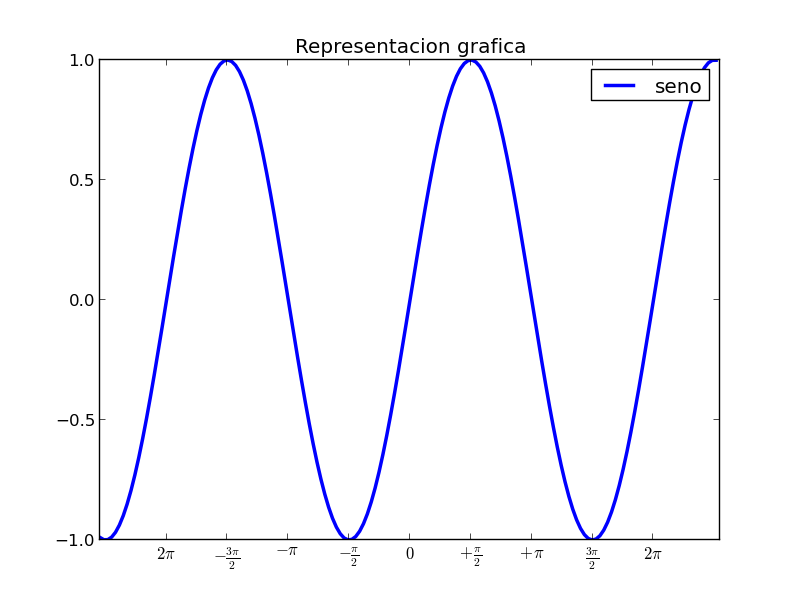
\includegraphics[width=0.75\textwidth]{images/grafico.eps}
\caption{Gr�fica de la funci�n original}
\label{fig:1}
\end{center}
\end{figure}
%------------------------------------------------------------------------------


%------------------------------------------------------------------------------
\begin{table}[!ht]
\begin{center}
\begin{tabular}{|l|c|c|c|c|c|}
\hline
Grado  & Punto c & Punto de Evaluacion & Aproximacion       & Error             & Tiempo CPU           \\ \hline
4      &   0.0   &    1                & 0.833333           & -0.833333         & 0.007406949996948242 \\ \hline
6      &   10    &    5                & 12.4605618963148   & -13.0045830072041 & 0.009202957153320312 \\ \hline
10     &   10    &    10               & -0.544021110889370 & 0                 & 0.010988950729370117  \\ \hline
\end{tabular}
\end{center}
\caption{Tabla de datos obtenidos experimentalmente}
\label{tab}
\end{table}

%------------------------------------------------------------------------------

%++++++++++++++++++++++++++++++++++++++++++++++++++++++++++++++++++++++++++++++
\section{An�lisis de los resultados}
\label{3:sec:4}

bla, bla, etc. 

